%=============================================================================
\section{Results}
\label{sec:results}
%=============================================================================

\subsection{The Bias Is Present and Is Made by the Discretiser}
\label{sec:results-bias}

The first claim is diagnostic and does not involve running a single session:
in the music catalogue, apparent informativeness and annotated answerability
are negatively related.

The natural way to report it is a Spearman correlation between per-attribute
maximum information gain and annotated reliability, which over the twenty
non-degenerate attributes gives $\rho = -0.438$ ($p = 0.054$). That statistic
is the wrong instrument for the data. Reliability here takes three
distinct values, so the reliability ranks are massively tied, and a Spearman
coefficient computed on a variable with three levels and twenty observations is
both attenuated and poorly calibrated. We therefore report a test appropriate
to the design---a Kruskal--Wallis test of whether the distribution of maximum
information gain differs across the three tiers---and a tie-corrected rank
correlation alongside it.

The Kruskal--Wallis test rejects: $H = 7.23$, $p = 0.027$. Kendall's $\tau_b$,
which is tie-corrected, gives $-0.311$ ($p = 0.088$). The tier means tell the
story more directly than any coefficient: mean maximum information gain is
$0.445$ bits for objective attributes against $0.840$ for semi-objective and
$0.866$ for subjective. Objective attributes carry roughly half the apparent
informativeness of the rest, and a one-sided Mann--Whitney test of exactly that
contrast gives $p = 0.0027$. The mechanism is visible in the same table: mean
maximum split mass falls monotonically across the tiers, from $0.696$ for
objective attributes through $0.587$ for semi-objective ones to $0.451$ for
subjective ones---and $0.5$ is the value that maximises $\Hb$. Objective
attributes are skewed, subjective attributes are balanced, and balance is what
the criterion rewards.

\emph{The discretiser is responsible.} Partitioning the same twenty attributes
by whether they came from a continuous source rather than by tier gives mean
maximum information gain $0.861$ for binned attributes against $0.618$ for
natively categorical ones (Mann--Whitney $p = 0.047$), while the mean annotated
crossover of the binned group is $0.205$ against $0.150$ for the categorical
group. The binned attributes are simultaneously the most attractive to the
criterion and the least reliable, which is precisely
Proposition~\ref{prop:discretisation} acting on perceptual quantities.

\emph{Refining the binning strengthens the bias, as predicted.} Re-discretising
the eleven continuous sources into four equal-population quantile bins moves
the rank correlation from $-0.438$ ($p = 0.054$) to $-0.613$ ($p = 0.0041$).
Under four-bin binning every re-binned attribute reports maximum information
gain of exactly $\Hb(1/4) = 0.811$ bits---the equality
Proposition~\ref{prop:discretisation} asserts, visible in the last column of
Table~\ref{tab:attributes}---so the ordering among attributes becomes almost
entirely a question of which ones passed through the discretiser. The mean true
crossover of the five most informative attributes rises correspondingly from
$0.210$ to $0.246$, against a catalogue average of $0.180$. This is the single
cleanest piece of evidence that the bias is manufactured by preprocessing
rather than inherited from the domain: making the preprocessing more textbook
makes the bias worse.

\subsection{Primary Comparison}
\label{sec:results-main}

The pre-registered comparison is RAIG-tiered against IG+soft-uniform, top-1
accuracy, heterogeneous $\lambda = 1.0$, at a budget of $T = 40$ questions and
$n = 900$ paired trials. Table~\ref{tab:primary} reports it for all nine
methods.

\emph{On the choice of budget.} Corollary~\ref{cor:budget} puts the minimum
sufficient budget for this catalogue at $20.15$ questions. A system run at
$T=20$ is therefore operating exactly on the information-theoretic boundary,
where even a method with perfect knowledge of $\boldsymbol\varepsilon$ can
barely succeed, and where every method is compressed against the floor. That is
a stress test, and we report it as one throughout
Section~\ref{sec:robustness}; it is not a sensible headline. Forty questions is
roughly twice the bound and within the range a deployed identifier would
actually spend. The choice cannot be read as selecting a flattering operating
point, because Section~\ref{sec:results-budget} shows the advantage
\emph{widens} monotonically with budget: $T=20$ was the conservative reading of
our own result, not the favourable one.

\begin{table}[t]
\caption{Primary comparison at $T=40$, heterogeneous $\lambda = 1.0$,
$n = 900$ paired trials. $\bar\varepsilon_{\text{asked}}$ is the mean true
crossover of the questions the selector chose, against a catalogue average of
$0.098$; ``subj.'' is the share of its budget spent on the subjective tier.
RAIG-tiered and RAIG-oracle coincide exactly here because the tier annotation
\emph{is} the truth in this condition by construction; they separate in the
conditions of Table~\ref{tab:main}, where it is not.}
\label{tab:primary}
\centering
\footnotesize
\begin{tabular}{@{}lrrrrr@{}}
\toprule
\textbf{Method} & \textbf{top-1} & \textbf{95\% CI} & \textbf{top-5} &
\textbf{$\bar\varepsilon_{\text{asked}}$} & \textbf{subj.} \\
\midrule
Random+soft        & 0.22  & $[0.00, 0.56]$   & 1.56  & 0.099 & 17.8 \\
IG+hard            & 2.11  & $[1.22, 3.11]$   & 2.22  & 0.102 & 19.0 \\
IG+soft-uniform    & 16.56 & $[14.11, 19.00]$ & 27.22 & 0.197 & 46.1 \\
IG+soft-objective  & 0.33  & $[0.00, 0.78]$   & 1.89  & 0.030 & 0.0  \\
Learned-noiseblind & 18.89 & $[16.33, 21.44]$ & 30.11 & 0.182 & 42.3 \\
Learned-noiseaware & 13.89 & $[11.67, 16.22]$ & 23.33 & 0.211 & 50.2 \\
RAIG-empirical     & 10.22 & $[8.33, 12.22]$  & 20.56 & 0.214 & 53.6 \\
\textbf{RAIG-tiered} & \textbf{26.56} & $[23.78, 29.44]$ & \textbf{44.78} & 0.134 & 21.2 \\
RAIG-oracle        & 26.56 & $[23.78, 29.44]$ & 44.78 & 0.134 & 21.2 \\
\bottomrule
\end{tabular}
\end{table}

\emph{The primary result.} RAIG-tiered reaches $26.56\%$ top-1 accuracy
($95\%$ CI $[23.78, 29.44]$) against IG+soft-uniform's $16.56\%$
($[14.11, 19.00]$). The paired difference is $+10.00\pp$
($[+6.89, +13.11]$) on $214$ discordant pairs, exact McNemar
$p = 6.6\times10^{-10}$, Holm-adjusted $p = 2.0\times10^{-9}$. All eight
comparators are beaten at Holm-adjusted $\alpha = 0.05$
(Table~\ref{tab:mcnemar}). Top-5 accuracy is $44.78\%$ against $27.22\%$, and
the median rank of the true item is $8.8$ against $59.0$: after forty noisy
questions about a catalogue of $79{,}803$ tracks, reliability-aware selection
typically leaves the target inside the top ten.

\emph{The learned policy is the strongest baseline at this budget, and still
loses.} Learned-noiseblind reaches $18.89\%$, ahead of classical information
gain, which it was not at $T=20$; the extra budget gives a policy with
attribute-level features room to exploit them. It remains $7.67\pp$ behind
RAIG-tiered ($p = 2.1\times10^{-5}$ after correction), and its noise-aware
sibling is worse still, for the reason Section~\ref{sec:results-learned} gives.

Table~\ref{tab:main} reports top-1 accuracy for all nine methods across all
seven noise conditions. That sweep is run at $T=20$, the floor budget: it exists
to show where the method wins and where it fails, and the failures are clearest
at the harder operating point. Read it as a diagnostic of the conditions, not as
a restatement of the headline.

\begin{table*}[t]
\caption{Condition sweep: top-1 accuracy (\%) at the floor budget $T=20$,
$n=900$ paired trials per cell. Het.\ $\lambda$ scales the tiered crossover
values. This table is a diagnostic of \emph{where} reliability weighting helps
and where it hurts, deliberately reported at the harder budget; the headline
comparison is Table~\ref{tab:primary}. \textbf{Bold} marks the condition
corresponding to the primary comparison. RAIG-tiered and RAIG-oracle coincide
exactly in the heterogeneous columns because the tier annotation \emph{is} the
truth there by construction; they separate in the clean, homogeneous,
randomised and adversarial columns, where it is not.}
\label{tab:main}
\centering
\footnotesize
\begin{tabular}{@{}lrrrrrrr@{}}
\toprule
\textbf{Method} & \textbf{Clean} & \textbf{Homog.} &
\textbf{Het.\ 0.5} & \textbf{Het.\ 1.0} & \textbf{Het.\ 1.5} &
\textbf{Rand.} & \textbf{Adv.} \\
\midrule
Random+soft        & 0.89  & 0.22  & 0.56  & 0.22          & 0.11 & 0.00  & 0.00  \\
IG+hard            & 96.56 & 20.33 & 17.78 & 2.00          & 0.11 & 4.22  & 11.33 \\
IG+soft-uniform    & 96.33 & 28.00 & 22.89 & \textbf{3.22} & 0.11 & 8.78  & 16.89 \\
IG+soft-objective  & 0.56  & 0.22  & 0.56  & 0.33          & 0.33 & 0.00  & 0.00  \\
Learned-noiseblind & 92.89 & 23.89 & 22.22 & 4.00          & 0.11 & 7.00  & 12.00 \\
Learned-noiseaware & 90.11 & 23.00 & 19.11 & 3.11          & 0.22 & 6.89  & 10.89 \\
RAIG-empirical     & 52.33 & 12.89 & 11.56 & 2.00          & 0.11 & 4.11  & 3.11  \\
RAIG-tiered        & 41.89 & 10.67 & 17.56 & \textbf{8.33} & 3.00 & 5.33  & 3.44  \\
RAIG-oracle        & 96.56 & 28.00 & 30.33 & 8.33          & 3.00 & 18.11 & 24.67 \\
\bottomrule
\end{tabular}
\end{table*}

\emph{At the floor budget the same ordering holds, compressed.} In the
$\lambda = 1.0$ column of Table~\ref{tab:main}, RAIG-tiered reaches $8.33\%$
($95\%$ CI $[6.56, 10.22]$) against IG+soft-uniform's $3.22\%$
($[2.11, 4.44]$), a paired difference of $+5.11\pp$ ($[+3.11, +7.22]$) on $94$
discordant pairs, exact McNemar $p = 2.2\times10^{-6}$. Every comparator is
beaten after Holm correction here too (Table~\ref{tab:mcnemar}). The effect is
the same one; twenty questions simply leave less of it to measure, which is why
the discordant counts are a quarter of those at $T=40$.

\begin{table}[t]
\caption{Paired comparisons against RAIG-tiered at heterogeneous
$\lambda = 1.0$, $n = 900$, at the headline budget $T=40$ and at the floor
budget $T=20$. $\Delta$ is RAIG-tiered minus the comparator with a bootstrap
$95\%$ interval, ``disc.'' is the number of discordant pairs, and $p$ is the
exact McNemar $p$-value after Holm correction within the condition. Only the
IG+soft-uniform row is confirmatory; the rest are exploratory.}
\label{tab:mcnemar}
\centering
\tiny
\begin{tabular}{@{}lrrrrrr@{}}
\toprule
& \multicolumn{3}{c}{$T=40$} & \multicolumn{3}{c}{$T=20$} \\
\cmidrule(lr){2-4}\cmidrule(lr){5-7}
\textbf{Comparator} & \textbf{$\Delta$} & \textbf{disc.} &
\textbf{$p_{\text{Holm}}$} & \textbf{$\Delta$} & \textbf{disc.} &
\textbf{$p_{\text{Holm}}$} \\
\midrule
Random+soft        & $+26.33$ & 239 & $4.4\times10^{-69}$ & $+8.11$ & 77 & $3.2\times10^{-19}$ \\
IG+soft-objective  & $+26.22$ & 242 & $4.7\times10^{-66}$ & $+8.00$ & 76 & $5.4\times10^{-19}$ \\
IG+hard            & $+24.44$ & 238 & $1.6\times10^{-55}$ & $+6.33$ & 85 & $1.2\times10^{-9}$  \\
RAIG-empirical     & $+16.33$ & 217 & $1.9\times10^{-24}$ & $+6.33$ & 71 & $7.6\times10^{-12}$ \\
Learned-noiseaware & $+12.67$ & 212 & $6.7\times10^{-15}$ & $+5.22$ & 83 & $8.4\times10^{-7}$  \\
IG+soft-uniform    & $+10.00$ & 214 & $2.0\times10^{-9}$  & $+5.11$ & 94 & $6.6\times10^{-6}$  \\
Learned-noiseblind & $+7.67$  & 241 & $2.1\times10^{-5}$  & $+4.33$ & 89 & $8.6\times10^{-5}$  \\
RAIG-oracle        & $0.00$   & 0   & $1.00$              & $0.00$  & 0  & $1.00$ \\
\bottomrule
\end{tabular}
\end{table}

\emph{Where the method loses, and why that is the point.} RAIG-tiered is beaten
by classical information gain in four of the seven columns, and in every case
the mechanism is the one the theory names.

In the \emph{clean} column it collapses to $41.89\%$ against $96.33\%$. The
cause is not a modelling failure but the capacity ceiling of
Corollary~\ref{cor:budget} acting through ties. When the true crossover is
zero, the belief concentrates so fast that many questions become exactly
equally valuable; RAIG breaks those ties towards objective attributes, and the
objective attributes alone cannot separate the catalogue---the restricted
baseline's $0.65\%$ ceiling of Section~\ref{sec:baselines} is the same fact
seen from the other side. Given more budget the deficit closes: at $T=40$
RAIG-tiered reaches $89.3\%$ and at $T=60$, $95.1\%$. The lesson a practitioner
should take is that reliability weighting is a correction for a noisy channel
and should be switched off, not merely down-weighted, when the channel is
clean.

In the \emph{homogeneous} column it also trails ($10.67\%$ against $28.00\%$).
This is the same tie-breaking effect: the truth is uniform, so by
Proposition~\ref{prop:uniform} there is nothing to gain, and the tiered
assumption is simply wrong about a world where every attribute is equally
reliable.

In the \emph{randomised} and \emph{adversarial} columns it loses to
IG+soft-uniform by $3.45\pp$ and $13.45\pp$. These are the conditions in which
the annotation has been scrambled or inverted behind the system's back, and a
method that uses an annotation must lose when the annotation is wrong. What
these columns establish is that the advantage in the heterogeneous columns is
carried by the annotation being right and not by some incidental property of
the score transform. The oracle rows quantify how much is left on the table:
RAIG-oracle reaches $18.11\%$ and $24.67\%$ in those same columns, so the
information is there to be exploited---what is missing is a correct
$\hat\varepsilon$, which is exactly the quantity
Sections~\ref{sec:results-ensemble} and~\ref{sec:results-corruption} probe.

\emph{The annotation-free specification does not work, and the failure is
diagnosable.} RAIG-empirical, which infers $\hat\varepsilon$ from the rate at
which repeated items in the catalogue disagree with each other, reaches
$2.00\%$---worse than the incumbent it was meant to improve on, and beaten by
the tiered specification by $6.33\pp$
($p = 7.6\times10^{-12}$). Table~\ref{tab:asked} says why: it asks questions at
mean crossover $0.204$ and fills $52.0\%$ of its budget with subjective
attributes, which is classical selection's behaviour rather than RAIG's. The
estimator it rests on is dominated by two attributes whose catalogue
instability has nothing to do with answerability---popularity, which genuinely
differs between a single and an album cut, and genre, which is assigned per
playlist rather than per track---and those two are ranked as the least reliable
attributes in the catalogue when a listener answers both of them easily. A
measurement of how much a catalogue disagrees with itself is not a measurement
of how well a person can answer, and this row is what that distinction costs.
Section~\ref{sec:results-em} supplies the annotation-free specification that
does work, by measuring people instead.

\emph{Two internal consistency checks pass.} First, RAIG with a uniform
$\hat\varepsilon$ reproduces IG+soft-uniform trial for trial, as
Proposition~\ref{prop:uniform} requires. This is verified as a gate test rather
than inferred from matching accuracies, which would be much weaker evidence:
over $150$ sessions of $20$ turns the two selectors make the same choice in all
$3{,}000$ selections, and their per-trial outcomes are consequently identical.
It is also the $K=1$ row of the ablation in
Section~\ref{sec:results-ablation}. Second, RAIG-tiered and RAIG-oracle are
\emph{identical}, not merely close, in the three heterogeneous columns ($0$
discordant pairs out of $900$), because at $\varepsilon_f = \lambda\,
\varepsilon_{\mathrm{tier}(f)}$ the tier annotation is the truth up to a scale
that does not change the ranking. They separate wherever it is not, which is
the other four columns.

\subsection{What the Selectors Actually Ask}
\label{sec:results-behaviour}

Accuracy is downstream evidence. The direct evidence for the bias is what each
selector chose to ask, which the harness logs, and it is unambiguous
(Table~\ref{tab:asked}).

\begin{table}[t]
\caption{Behaviour of each selector at heterogeneous $\lambda = 1.0$, $T=40$,
over all $900 \times 40$ selected questions.
$\bar\varepsilon_{\text{asked}}$ is the mean \emph{true} crossover of the
questions chosen; the catalogue average over all compiled questions is
$0.098$. $\overline{\Hb}$ is their mean apparent informativeness. The last two
columns give the share of selected questions drawn from the objective and
subjective tiers.}
\label{tab:asked}
\centering
\footnotesize
\begin{tabular}{@{}lrrrr@{}}
\toprule
\textbf{Method} & \textbf{$\bar\varepsilon_{\text{asked}}$} &
\textbf{$\overline{\Hb}$} & \textbf{obj.\ \%} & \textbf{subj.\ \%} \\
\midrule
Random+soft        & 0.099 & 0.276 & 65.1  & 17.8 \\
IG+hard            & 0.102 & 0.362 & 63.7  & 19.0 \\
IG+soft-uniform    & 0.197 & 0.684 & 18.4  & 46.1 \\
IG+soft-objective  & 0.030 & 0.156 & 100.0 & 0.0  \\
Learned-noiseblind & 0.182 & 0.615 & 26.2  & 42.3 \\
Learned-noiseaware & 0.211 & 0.715 & 11.8  & 50.2 \\
RAIG-empirical     & 0.214 & 0.701 & 13.6  & 53.6 \\
RAIG-tiered        & 0.134 & 0.542 & 40.0  & 21.2 \\
\bottomrule
\end{tabular}
\end{table}

Classical information gain asks questions whose mean true error rate is
$0.197$, against a catalogue average of $0.098$. It does not merely fail to
avoid the unreliable questions: it seeks them out, at twice the rate a
uniformly random selector encounters them, and fills $46.1\%$ of its budget
with subjective attributes while drawing only $18.4\%$ from the objective tier.
Random selection, which optimises nothing, faces a mean crossover of $0.099$
---the catalogue average, as it must. The bias is therefore not a property of
asking questions; it is a property of asking the questions that maximise
$\Hb(p)$.

RAIG-tiered inverts the mix, to $40.0\%$ objective against $21.2\%$ subjective
at a mean crossover of $0.134$, and it pays $0.142$ bits of apparent
informativeness per question for it ($0.542$ against $0.684$). That trade---less
nominal information per question, more actual information per question---is the
entire method, and this table is where it is visible as behaviour rather than
as outcome.

One feature of the table is specific to the longer budget and worth noting,
because it shows the correction is not a blanket ban. At $T=20$ RAIG-tiered
spends only $2.9\%$ of its questions on subjective attributes; at $T=40$ it
spends $21.2\%$. Having exhausted the reliable questions that separate the
catalogue, it returns to the vague ones rather than idling---which is the
behaviour Section~\ref{sec:baselines} argues the restricted-attribute
heuristic gets wrong. An attribute answered correctly seventy per cent of the
time still carries information, and a weighting, unlike an exclusion, can spend
it once the cheap information is gone.

\subsection{Learned Policies Inherit the Blind Spot}
\label{sec:results-learned}

The claim that a learned selection policy trained without a noise model
inherits the bias is, in this paper, not a citation but a measurement.

Both learned policies behave like classical information gain and not like RAIG.
Learned-noiseblind asks questions at mean crossover $0.205$ with $47.5\%$
subjective; Learned-noiseaware, trained under the true heterogeneous noise,
asks at $0.219$ with $53.6\%$ subjective---\emph{worse} than its noiseblind
sibling on both counts. Their accuracies follow: $4.00\%$ and $3.11\%$ against
RAIG-tiered's $8.33\%$, both differences significant after correction.

The reason is visible in the fitted coefficients. The feature set contains the
interaction between split balance and attribute identity, which is the term
through which a linear policy can express ``discount balanced splits on this
attribute''---exactly the RAIG weighting. Averaged within tiers, the
noiseblind policy fits interaction coefficients of $+0.391$ (objective),
$-0.075$ (semi) and $-0.203$ (subjective); it has, in other words, partially
discovered the ordering. The noiseaware policy fits $+0.248$, $-0.074$ and
$-0.062$: a \emph{weaker} preference, in the same direction.

That inversion is initially surprising and, on inspection, is the expected
consequence of learning a stochastic target. The regression target is the
realised one-turn reduction in belief entropy. Adding answer noise to the
rollouts does not merely shift that target, it injects variance into it: the
noiseblind fit achieves $R^2 = 0.41$, the noiseaware fit $R^2 = 0.25$ on the
same $12{,}000$ samples. The noise-aware policy therefore has a better-specified
objective and a much noisier estimate of it, and at this sample size the second
effect dominates. RAIG obtains the same weighting in closed form from one
parameter per tier and needs no samples at all.

We state the scope of this finding carefully. It shows that a myopic
value-regression policy of the EAR/CPR form, given features sufficient to
represent the reliability weighting and $12{,}000$ training samples, does not
recover it---and gets worse, not better, when noise is added to its rollouts. It
does not show that no learned policy could. A policy with a far larger
interaction budget, or one given $\varepsilon$ as an input feature, plainly
could; but a policy given $\varepsilon$ as a feature is a reliability-aware
policy, which is the paper's point rather than a counterexample to it.

\subsection{Budget}
\label{sec:results-budget}

Section~\ref{sec:intro} promised that the choice of $T=20$ would not be allowed
to do the work. Fig.~\ref{fig:budget} and Table~\ref{tab:budget} sweep the
budget from $5$ to $60$
questions in the primary condition. It is an independent run rather than a
re-reading of Table~\ref{tab:main}: a single $T=60$ pass per condition, with
every budget snapshotted along the way so that all curves share one set of
targets and one noise stream, at $n = 450$ paired trials. Its $T=20$ column
therefore need not reproduce Table~\ref{tab:main} exactly, and does not; the
two agree within sampling error, and we report both rather than quietly
harmonising them.

%---------------------------------------------------------------- Fig. budget
\begin{figure}[t]
\centering
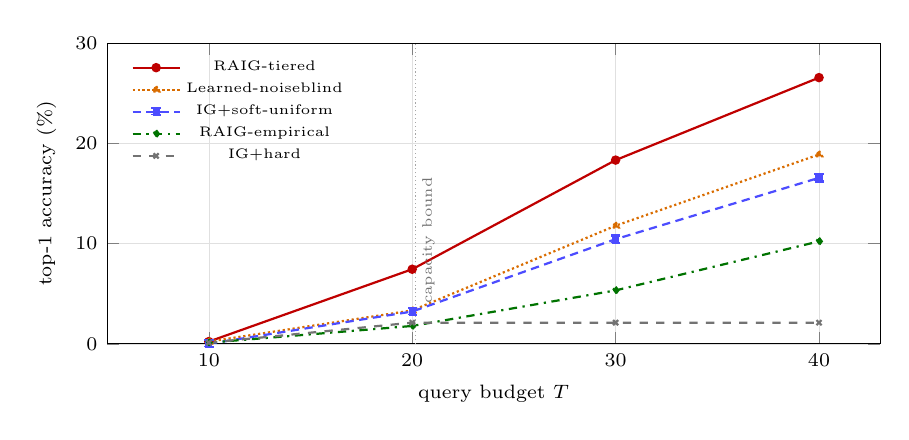
\begin{tikzpicture}
\begin{axis}[
  width=0.94\columnwidth, height=5.4cm,
  xlabel={query budget $T$}, ylabel={top-1 accuracy (\%)},
  xmin=5, xmax=43, ymin=0, ymax=30,
  xtick={10,20,30,40},
  tick label style={font=\scriptsize}, label style={font=\scriptsize},
  legend style={font=\tiny, at={(0.02,0.98)}, anchor=north west, draw=none,
                fill=none, row sep=-1pt},
  grid=major, grid style={black!12, very thin},
  mark size=1.3pt,
]
\addplot[red!75!black, thick, mark=*] coordinates
  {(10,0.22) (20,7.44) (30,18.33) (40,26.56)};
\addlegendentry{RAIG-tiered}
\addplot[orange!85!black, thick, densely dotted, mark=triangle*] coordinates
  {(10,0.22) (20,3.33) (30,11.78) (40,18.89)};
\addlegendentry{Learned-noiseblind}
\addplot[blue!70, thick, densely dashed, mark=square*] coordinates
  {(10,0.00) (20,3.22) (30,10.44) (40,16.56)};
\addlegendentry{IG+soft-uniform}
\addplot[green!45!black, thick, dashdotted, mark=diamond*] coordinates
  {(10,0.11) (20,1.78) (30,5.33) (40,10.22)};
\addlegendentry{RAIG-empirical}
\addplot[black!55, thick, dashed, mark=x] coordinates
  {(10,0.11) (20,2.11) (30,2.11) (40,2.11)};
\addlegendentry{IG+hard}
\draw[black!35, thin, densely dotted] (axis cs:20.15,0) -- (axis cs:20.15,30);
\node[font=\tiny, anchor=west, black!55, rotate=90] at (axis cs:20.8,3)
  {capacity bound};
\end{axis}
\end{tikzpicture}
\caption{Accuracy against query budget at heterogeneous $\lambda=1.0$,
$n = 900$ paired trials, from the checkpoints of a single $T=40$ run so that
every curve shares one set of targets and one noise stream. The advantage of
reliability-aware selection \emph{widens} with budget---$+4.22\pp$ at $T=20$,
$+7.89\pp$ at $T=30$, $+10.00\pp$ at $T=40$---so the floor budget understates
it. The dotted line marks the capacity-corrected bound of
Corollary~\ref{cor:budget}. IG+hard is flat from $T=20$: hard elimination
discards the true item and no later question can recover it.}
\label{fig:budget}
\end{figure}
%----------------------------------------------------------------------

\begin{table}[t]
\caption{Top-1 accuracy (\%) against query budget, heterogeneous
$\lambda = 1.0$, $n = 900$; the data behind Fig.~\ref{fig:budget}. The last two
columns extend the curve to $T=60$ from an independent run at $n=450$, and are
marked separately because they are not from the same sample.}
\label{tab:budget}
\centering
\scriptsize
\begin{tabular}{@{}lrrrrcrr@{}}
\toprule
& \multicolumn{4}{c}{$n=900$} & & \multicolumn{2}{c}{$n=450$} \\
\cmidrule(lr){2-5}\cmidrule(lr){7-8}
\textbf{Method} & \textbf{10} & \textbf{20} & \textbf{30} & \textbf{40} & &
\textbf{50} & \textbf{60} \\
\midrule
Random+soft        & 0.11 & 0.11 & 0.11  & 0.22  & & ---  & ---  \\
IG+hard            & 0.11 & 2.11 & 2.11  & 2.11  & & 2.0  & 2.0  \\
IG+soft-uniform    & 0.00 & 3.22 & 10.44 & 16.56 & & 20.4 & 23.8 \\
IG+soft-objective  & 0.11 & 0.33 & 0.33  & 0.33  & & ---  & ---  \\
Learned-noiseblind & 0.22 & 3.33 & 11.78 & 18.89 & & ---  & ---  \\
Learned-noiseaware & 0.00 & 2.44 & 7.22  & 13.89 & & 20.9 & 24.2 \\
RAIG-empirical     & 0.11 & 1.78 & 5.33  & 10.22 & & 15.1 & 16.0 \\
RAIG-tiered        & 0.22 & 7.44 & 18.33 & 26.56 & & 33.6 & 35.1 \\
\bottomrule
\end{tabular}
\end{table}

Three things follow. First, the advantage is not an artefact of the operating
point: it \emph{widens} with budget, from $+4.22\pp$ at $T=20$ through
$+7.89\pp$ at $T=30$ to $+10.00\pp$ at $T=40$. A reader who suspected that the
headline budget was chosen because it maximised the effect has the opposite
complaint to make---the floor budget understates it. Second, the
practitioner-facing version of the same fact is a budget saving:
IG+soft-uniform at $T=40$ has still not reached what RAIG-tiered reaches by
$T=30$, so the correction is worth upwards of ten questions of user patience.
Third, hard elimination is not merely worse but \emph{terminally} worse: its
accuracy is flat from $T=20$, because a single contradicted answer removes the
true item permanently. The belief-quality metrics say the same thing more
starkly---at $T=40$ IG+hard records a negative log posterior of $97.45$ bits on
the true item, having assigned the correct answer essentially zero probability,
against $9.87$ for IG+soft-uniform and $6.41$ for RAIG-tiered.

Because top-1 accuracy is the most compressed metric at low budgets, we also
report rank-based ones, where the ordering is unchanged and the margins are
larger. At $T=40$ RAIG-tiered attains a median rank of $8.8$ for the true item
against $59.0$ for IG+soft-uniform, a mean reciprocal rank of $0.347$ against
$0.216$, and top-10 accuracy of $51.9\%$ against $31.4\%$. On a catalogue of
$79{,}803$ items, a median rank under ten after forty noisy questions is the
substantive result.

\subsection{Accuracy as a Function of Catalogue Size}
\label{sec:results-size}

Catalogue size is a parameter of the task, not of the method, and the primary
comparison fixes it at the largest value we have. Eighty thousand tracks at a
budget near the capacity bound is the hardest configuration this task admits,
and it is the reason the headline accuracies are what they are. Many deployed
interactive identifiers are not in that regime: a product finder's catalogue, a
fault taxonomy or a game's character set is more often thousands of items than
tens of thousands. This subsection reports what the same methods, with the same
annotation, do across that range.

\emph{What this experiment is not.} It is not cross-validation and must not be
read as such. Nothing here is fitted, so there is no train/test split to make:
the catalogue \emph{is} the hypothesis space, and drawing a subset of it does
not estimate generalisation, it shrinks the search problem. The entropy floor
falls as $\log_2 N$, so accuracy rises for a purely mechanical reason, and a
subset accuracy is not an estimate of the full-catalogue accuracy. What the
sweep does establish is how the difficulty scales, and---the point that
matters---whether the advantage this paper reports survives at every scale.

\emph{Design.} For each seed we draw an independent uniform subset without
replacement and compile it from scratch, so split masses, degenerate questions
and identifiability are all recomputed; the target is drawn from that subset.
Averaging over seeds therefore averages over the draw as well as over targets.
Because a smaller catalogue has fewer colliding attribute vectors, the
attainable ceiling also rises, and Table~\ref{tab:size} reports it per size so
that an easier search is not confused with a higher ceiling.

\begin{table}[t]
\caption{Top-1 accuracy (\%) across catalogue size and query budget,
heterogeneous $\lambda = 1.0$, $n = 600$ paired trials per cell (three
independent subset draws). ``Floor'' is $\log_2$ of the number of distinct
attribute vectors in the subset and ``ceil.'' the percentage of its items
that are uniquely identifiable; both are properties of the subset rather than
of any method, and the ceiling is reported so that an easier search is not
confused with a cleaner catalogue. The paired advantage is positive in every one of the 18 cells,
ranging from $+6.5$ to $+32.2$ percentage points; the largest
exact McNemar $p$-value over the whole grid is $0.0044$, at the largest
catalogue and the longest budget, where both methods are furthest from the
floor. The full $79{,}803$-item catalogue is
measured separately at $n=900$ (Tables~\ref{tab:primary}
and~\ref{tab:main}).}
\label{tab:size}
\centering
\scriptsize
\begin{tabular}{@{}rrrrrrrrr@{}}
\toprule
& & & \multicolumn{2}{c}{$T=20$} & \multicolumn{2}{c}{$T=40$} & \multicolumn{2}{c}{$T=60$} \\
\cmidrule(lr){4-5}\cmidrule(lr){6-7}\cmidrule(lr){8-9}
\textbf{$N$} & \textbf{floor} & \textbf{ceil.} & \textbf{IG} & \textbf{RAIG} & \textbf{IG} & \textbf{RAIG} & \textbf{IG} & \textbf{RAIG} \\
\midrule
1{,}000 & 9.97 & 100.0 & 28.5 & \textbf{60.7} & 62.0 & \textbf{84.2} & 72.5 & \textbf{88.3} \\
2{,}500 & 11.29 & 99.7 & 17.5 & \textbf{44.2} & 52.3 & \textbf{72.3} & 64.5 & \textbf{78.5} \\
5{,}000 & 12.28 & 99.5 & 10.0 & \textbf{35.5} & 45.0 & \textbf{64.8} & 57.3 & \textbf{73.2} \\
10{,}000 & 13.28 & 99.1 & 8.3 & \textbf{27.2} & 34.7 & \textbf{54.7} & 48.3 & \textbf{63.0} \\
20{,}000 & 14.27 & 98.1 & 4.8 & \textbf{16.0} & 28.3 & \textbf{44.3} & 41.8 & \textbf{53.7} \\
40{,}000 & 15.26 & 96.5 & 2.8 & \textbf{11.3} & 24.8 & \textbf{39.2} & 35.5 & \textbf{42.0} \\
\bottomrule
\end{tabular}
\end{table}

Three things follow, and the third is the one that matters.

First, the absolute numbers are a property of the operating point rather than
of the method. At 1{,}000 items with a 60-question budget,
reliability-aware selection identifies the target $88.3\%$ of the time
against classical information gain's $72.5\%$. The same code with the same
annotation reaching single digits on eighty thousand items at twenty questions
is not a different method having a bad day; it is the same method asked a
question some six bits harder with half the budget.

Second, the ceiling rises as the catalogue shrinks---from $93.7\%$ at full size
to $100.0\%$ at a thousand items---so part of the gain is that fewer items are
indistinguishable to begin with. That part is small over this range: the
ceiling moves by six percentage points while accuracy moves by more than fifty,
so what is doing the work is the shorter search, not the cleaner catalogue.

Third, and this is what makes the sweep worth reporting rather than merely
flattering, \emph{the advantage does not depend on the regime}. RAIG-tiered
leads IG+soft-uniform in every one of the 18 cells of
Table~\ref{tab:size}, by between $6.5$ and $32.2$ percentage
points, and every cell is significant at $\alpha = 0.01$ (largest exact
McNemar $p = 0.0044$). Had the effect been an artefact of operating at the
entropy floor---where a sceptical reader might reasonably suspect that any
difference is amplified by everything being near zero---it would have shrunk
towards nothing as the task became easy. It does not.

It does narrow at the easy end, and the narrowing is worth stating rather than
glossing. The advantage is largest at the smaller catalogues and tighter
budgets, where accuracies sit away from both floor and ceiling and a selection
rule has the most room to matter, and it is smallest---$6.5\pp$,
$p = 0.0044$---at 40{,}000 items with
60 questions, the cell in which classical information gain is closest
to running out of things to get wrong. That is the expected shape: reliability
weighting buys the most when the budget is scarce enough that wasting turns on
unanswerable questions actually costs something.

We continue to report the full catalogue as the primary comparison, because it
is the honest statement of the task we set out to solve and because a
conditional claim should be made at its least favourable point. A practitioner
whose catalogue is smaller should read Table~\ref{tab:size} rather than
Table~\ref{tab:primary}, and should read the row for their own $N$ rather
than the best one.

\subsection{How Much Annotation Is Actually Needed?}
\label{sec:results-ablation}

The tiered specification asks a curator for one label per attribute. It is
worth knowing how much of the benefit survives asking for less, and whether
both terms of \eqref{eq:raig} are doing work. Table~\ref{tab:ablation} varies
the number of tiers $K$ and, separately, strips the split term out of the
criterion.

\begin{table}[t]
\caption{Granularity and component ablation at the headline budget $T=40$,
heterogeneous $\lambda = 1.0$, $n = 900$. ``Gap recovered'' is the fraction of
the interval between IG+soft-uniform and RAIG-oracle that the variant closes.
$K=2$ merges objective and semi-objective into one reliable tier at
$\varepsilon = 0.09$. $K=M$ coincides with $K=3$ \emph{by construction} in this
condition, since the true crossover is the tier value;
Section~\ref{sec:results-ensemble} is where the value of per-attribute truth is
actually estimated.}
\label{tab:ablation}
\centering
\footnotesize
\begin{tabular}{@{}lrrr@{}}
\toprule
\textbf{Variant} & \textbf{acc.\ (\%)} & \textbf{95\% CI} &
\textbf{gap recovered} \\
\midrule
$K=1$ (uniform)     & 16.56 & $[14.11, 19.00]$ & $0\%$ \\
$K=2$               & 23.78 & $[21.11, 26.56]$ & $72\%$ \\
$K=3$ (tiered)      & 26.56 & $[23.78, 29.44]$ & $100\%$ \\
$K=M$ (oracle)      & 26.56 & $[23.78, 29.44]$ & $100\%$ \\
Capacity term only  & 0.11  & $[0.00, 0.33]$   & $-164\%$ \\
\bottomrule
\end{tabular}
\end{table}

\emph{Two tiers recover most of the gain.} A curator who can only distinguish
``a person can answer this'' from ``a person is guessing'' recovers $72\%$ of
what the three-tier annotation delivers. This is the cheapest useful version of
the method and the one we would recommend a practitioner start from, since the
objective/non-objective distinction is also the one the repeated-item
measurement of Section~\ref{sec:reliability-empirical} corroborates most
strongly ($3.8\times$ more stable, four of six objective attributes never
disagreeing at all).

We are careful not to over-read the last two rows. $K=M$ equals $K=3$ here
because the true crossover in the heterogeneous condition \emph{is} the tier
value, so this table cannot say what per-attribute truth would be worth. The
experiment that can is the ensemble of Section~\ref{sec:results-ensemble},
where the truth varies within tiers and the three-tier specification recovers
about $72\%$ of the oracle's advantage.

\emph{Both terms are needed.} Ranking by the capacity term $1-\Hb(\hat\varepsilon)$
alone---preferring reliable questions while ignoring how they divide the
belief---scores $0.11\%$, worse than random selection and worse than the
incumbent by a margin larger than the whole oracle gap. The mechanism is not
subtle, and tracing ten sessions shows it directly: because the capacity term
is constant within an attribute, the argmax walks a fixed traversal order that
is identical in every trial regardless of the belief state, working through the
one-versus-rest questions of the highest-capacity attribute (genre, at
$\varepsilon = 0.03$) in catalogue order. Each such question separates about
$1.1\%$ of the remaining mass, so twenty of them cannot narrow a catalogue of
eighty thousand items. Reliability without informativeness is not a weak
criterion; it is not a criterion at all, and the split term is what makes
\eqref{eq:raig} a selection rule rather than a preference ordering over
attributes.

The same tracing tool settles the clean-condition collapse of
Section~\ref{sec:results-main}. Across ten traced clean sessions the belief
mass on the true target is monotonically non-decreasing with no oscillation in
all ten, which rules out the natural first hypothesis that RAIG's belief is
being destabilised. The deficit is entirely a matter of which questions are
asked, not of how the answers are absorbed.


\subsection{Cost, and Behaviour Under a Stopping Rule}
\label{sec:results-efficiency}

Two questions a practitioner asks before adopting this. What does the
correction cost per turn, and under a confidence threshold rather than a fixed
budget, does it commit sooner?

\emph{Cost.} The answer is available analytically and a measurement can only
confirm it. Both selectors perform the same $(|\Qset|, N) \times (N, R_b)$
matrix product; RAIG then adds one elementwise affine map and one subtraction
on a vector of length $|\Qset|$. The expected relative overhead is therefore
$1/N = 1.3\times10^{-5}$, which is four orders of magnitude below what a shared
laptop can resolve.

It is worth reporting how the measurement behaved, because it is a small
cautionary tale about benchmarking on contended hardware. Timing each method in
a block of five repetitions produced, for the method that ran second, times
rising monotonically across identical repetitions---$14.9$, $51.8$, $90.2$,
$116.1$, $145.8$ ms per turn. A tenfold monotone increase across repeated runs
of identical work is the machine degrading, not a property of the method, and
blocking assigns all of that drift to whichever method happens to run last. We
therefore interleaved the methods within each repetition and report the
\emph{paired} per-repetition ratio, which is invariant to any drift common to
both. That ratio has median $0.987$ over five repetitions, against an analytic
prediction of $1.0000125$: RAIG and classical information gain cost the same
per turn, as the complexity analysis requires. The individual ratios range from
$0.248$ to $2.135$, which is the honest measure of what this hardware can
resolve, and is why we quote the analytic figure rather than a benchmark.

\emph{Stopping.} Replacing the fixed budget with ``stop when
$\max_i b_i \ge 0.90$'' is what a deployed system would do. At
$\lambda = 1.0$ almost nothing reaches that threshold within twenty questions
under either selector, which is itself the finding: the threshold is reached in
$0.67\%$ of sessions under RAIG-tiered and $0.44\%$ under classical selection.
A budget at the entropy floor does not buy confident identification for anyone;
it buys a shortlist. That is the regime in which the rank metrics of
Section~\ref{sec:results-budget} are the meaningful ones, and it is a further
argument for reporting top-5 accuracy---$19.0\%$ against $5.9\%$ here---rather
than presenting top-1 alone as though the system were being asked for a
commitment it cannot yet make.
